\documentclass[mathserif,compress,xcolor={dvipsnames}]{beamer}

\mode<presentation>
{
  \usecolortheme{orchid}
  \useoutertheme{shadow}
}
\newcommand\hmmax{0}
\newcommand\bmmax{0}
\usepackage{natbib, verbatim}

\usepackage[utf8]{inputenc}

\usepackage{mathpazo}
\usepackage[T1]{fontenc}

\usepackage{amsmath}
\usepackage{amsthm}
\usepackage{amssymb}
\usepackage{blkarray}
\usepackage{mathptmx}
\usepackage{anyfontsize}
\usepackage{t1enc}
\usepackage{appendix}
\usepackage{array}
\usepackage{bm}
\usepackage{cancel}
\usepackage{cite}
\usepackage{courier}
\usepackage{graphicx}
\usepackage{empheq}
\usepackage{enumerate}
\usepackage{listings}
\usepackage{mathtools}
\usepackage{units}
\usepackage{bigstrut}
\usepackage{rotating}
\usepackage{multirow}
\usepackage{booktabs}
\usepackage{algorithm, algorithmic}

\usepackage{lipsum}

\newcommand\Wider[2][3em]{%
\makebox[\linewidth][c]{%
  \begin{minipage}{\dimexpr\textwidth+#1\relax}
  \raggedright#2
  \end{minipage}%
  }%
}

\DeclareMathAlphabet{\mathcal}{OMS}{cmsy}{m}{n}

\DeclareMathAlphabet{\mathsfit}{\encodingdefault}{\sfdefault}{m}{}
\SetMathAlphabet{\mathsfit}{bold}{\encodingdefault}{\sfdefault}{bx}{}


\usepackage{color}
\lstset{language=R,basicstyle=\ttfamily,breaklines=true,
                keywordstyle=\color{blue}\ttfamily,
                stringstyle=\color{red}\ttfamily,
                commentstyle=\color{magenta}\ttfamily,
                showstringspaces=false,
                }

\newcommand*\widefbox[1]{\fbox{\hspace{2em}#1\hspace{2em}}}
\newcommand*\mb{\mathbf}
\newcommand*\reals{\mathbb{R}}
\newcommand*\complex{\mathbb{C}}
\newcommand*\naturals{\mathbb{N}}
\newcommand*\nats{\naturals}
\newcommand*\integers{\mathbb{Z}}
\newcommand*\rationals{\mathbb{Q}}
\newcommand*\irrationals{\mathbb{J}}
\newcommand*\pd{\partial}
\newcommand*\htab{\hspace{4 mm}}
\newcommand*\vtab{\vspace{0.5 in}}
\newcommand*\lsent{\mathcal{L}}
\newcommand*\conj{\overline}
\newcommand*\union{\cup}
\newcommand*\intersect{\cap}
\newcommand*\cl{\cancel}
\newcommand*\ANS{\text{ANS}}
\newcommand*\As{\text{As}}
\newcommand*\then{\rightarrow}
\newcommand*\elim{\text{E}}
\newcommand*\intro{\text{I}}
\newcommand*\absurd{\curlywedge}
\newcommand*\NK{\vdash_{\text{NK}}}
\newcommand*\derivation{\begin{tabular} { >{$}l<{$}  >{$}c<{$}  >{$}l<{$}  >{$}r<{$} }}
\newcommand*\interp{\mathcal{I}}
\newcommand*\ba{\[ \begin{aligned}}
\newcommand*\ea{\end{aligned} \]}
\newcommand*\C{\mathcal{C}}
\newcommand*\D{\mathscr{D}}
\newcommand*\e{\operatorname{e}}
\newcommand*\df{=_{\text{def}}}
\newcommand*\eps{\epsilon}
\newcommand*\enum{\begin{enumerate}[label=(\alph*)]}
\newcommand*\enumend{\end{enumerate}}
\newcommand*\E[1]{\mathsf{E}\left[#1\right]}
\newcommand*\Esub[2]{\mathsf{E}_{#1}\left[#2\right]}
\newcommand*\Var[1]{\mathsf{Var}\left[#1\right]}
\newcommand*\Cov[1]{\mathsf{Cov}\left[#1\right]}
\newcommand*\iid{\overset{\text{iid}}{\sim}}
\newcommand*\Exp[1][\lambda]{\text{Exp}(\text{rate}=#1)}
\newcommand*\ind[2]{I_{({#1}, {#2})} }
\newcommand*\set[1]{\left\{#1\right\}}
\newcommand*\estim[1]{\widehat{#1}}
\newcommand*\der{\text{d}}
\newcommand*\norm[1]{\left\|#1\right\|}
\newcommand*\dist[2]{\;\text{dist}\left(#1, #2\right)}
\newcommand*\interior{\text{int}\;}
\newcommand*\exterior{\text{ext}\;}
\newcommand*\boundary{\text{bd}\;}
\newcommand*\lh{\overset{\text{L'H}}{=}}

\renewcommand\Re{\operatorname{Re}}
\renewcommand\Im{\operatorname{Im}}
\DeclareMathOperator*{\argmin}{arg\;min}
\renewcommand\;{\,}
\renewcommand\epsilon{\varepsilon}
\renewcommand\rho{\varrho}
\renewcommand\phi{\varphi}
\renewcommand\mod{\hspace{0.2em} \textbf{mod}\hspace{0.2em}}
\renewcommand\Pr[1]{ \mathsf{Pr}\left(#1\right)}
\def\ci{\perp\!\!\!\perp}

\usepackage{tikz}
\usetikzlibrary{positioning}
\usetikzlibrary{shapes,arrows}
\usepackage{adjustbox}

\tikzstyle{decision} = [diamond, draw, fill=blue!20, 
    text width=4.5em, text badly centered, node distance=3cm, inner sep=0pt]
\tikzstyle{block} = [rectangle, draw, fill=blue!20, 
    text width=6em, text centered, rounded corners, minimum height=4em]
\tikzstyle{line} = [draw, -latex']
\tikzstyle{cloud} = [draw, ellipse,fill=red!20, node distance=3cm,
    minimum height=2em]

\lstset{breaklines=true,
        numbersep=5pt,
        xleftmargin=.25in,
        xrightmargin=.25in}

\DeclareMathOperator{\sech}{sech}
\DeclareMathOperator{\sgn}{sgn}
\makeatletter
\renewcommand*\env@matrix[1][*\c@MaxMatrixCols c]{%
  \hskip -\arraycolsep
  \let\@ifnextchar\new@ifnextchar
  \array{#1}}
\makeatother

\newenvironment{amatrix}[1]{%
  \left(\begin{array}{@{}*{#1}{c}|c@{}}
}{%
  \end{array}\right)
}

\lstset{basicstyle=\footnotesize\ttfamily,breaklines=true}


\newcommand{\real}{\ensuremath{\mathbb{R}}}
\newcommand{\bA}{\mbox{\protect\boldmath $A$}}
\newcommand{\bo}{\mbox{\protect\boldmath $o$}}
\newcommand{\bu}{\mbox{\protect\boldmath $u$}}
\newcommand{\by}{\mbox{\protect\boldmath $y$}}
\newcommand{\bx}{\mbox{\protect\boldmath $x$}}
\newcommand{\bs}{\mbox{\protect\boldmath $s$}}
\newcommand{\bS}{\mbox{\protect\boldmath $S$}}
\newcommand{\bz}{\mbox{\protect\boldmath $z$}}
\newcommand{\bh}{\mbox{\protect\boldmath $h$}}
\newcommand{\bF}{\mbox{\protect\boldmath $f$}}
\newcommand{\bt}{\mbox{\protect\boldmath $t$}}
\newcommand{\bc}{\mbox{\protect\boldmath $c$}}
\newcommand{\bC}{\mbox{\protect\boldmath $C$}}
\newcommand{\bV}{\mbox{\protect\boldmath $V$}}
\newcommand{\bX}{\mbox{\protect\boldmath $X$}}
\newcommand{\bW}{\mbox{\protect\boldmath $W$}}
\newcommand{\bZ}{\mbox{\protect\boldmath $Z$}}
\newcommand{\bof}{\mbox{\protect\boldmath $f$}}
\newcommand{\indicator}{{\ensuremath{\mathbb{I}}}}
\newcommand{\M}{{\ensuremath{\rm M}}}
\newcommand{\bbeta}{\boldsymbol{\beta}}
\newcommand{\balpha}{\boldsymbol{\alpha}}
\newcommand{\bgamma}{\boldsymbol{\gamma}}
\newcommand{\bdelta}{\boldsymbol{\delta}}
\newcommand{\btheta}{\boldsymbol{\theta}}
\newcommand{\bzero}{\mathbf{0}}
\newcommand{\hsp}{\hspace{0.2mm}}

\footnotesize

\beamertemplatenavigationsymbolsempty
\setbeamertemplate{headline}{\vskip2pt}

\title[]{T cell receptor repertoire comparison and motif discovery via optimal transport}

\author[]
{Branden Olson Steele}

\date[Jun 5, 2020]
{June 5, 2020}

\institute[]
{
Department of Statistics
\\
University of Washington Seattle
}

\AtBeginSection[]
{
   \begin{frame}
       \frametitle{Outline}
       \tableofcontents[currentsection]
   \end{frame}
}

\expandafter\def\expandafter\insertshorttitle\expandafter{%
  \insertshorttitle\hspace{22em}%
  \insertframenumber}

\begin{document}

\begin{frame}[noframenumbering]
  \titlepage
\end{frame}

\begin{frame}\frametitle{Cooking fun}
\includegraphics[width=0.8\linewidth]{Images/homity_pie.jpg}

\includegraphics[width=0.8\linewidth]{Images/halloumi.jpg}
\end{frame}

\section{Introduction to T cell receptors}

\begin{frame}\frametitle{T cell receptors (TCRs)}
\begin{center}
\includegraphics[width=0.6\linewidth]{Images/TCR.png}
\end{center}
\end{frame}

\begin{frame}\frametitle{TCRs and BCRs}
\begin{center}
\includegraphics[width=0.5\linewidth]{Images/bcr_tcr.png}
\end{center}
\end{frame}


\begin{frame}\frametitle{TCR repertoires}
\begin{itemize}
\item[]
A TCR \emph{repertoire} is the collection of TCRs in an individual at a given moment
\bigskip
\item[]
This changes in time
\bigskip
\item[]
Can sample via high-throughput sequencing
\end{itemize}
\end{frame}


\begin{frame}\frametitle{TCR distributions}
\begin{center}
\includegraphics[width=0.6\linewidth]{Images/transport-cartoon.png}
\end{center}
\end{frame}

\begin{frame}\frametitle{TCR repertoire comparison}
\begin{itemize}
\bigskip
\item
But comparing (and even visualizing) TCR distributions not quite straightforward...
\end{itemize}
\begin{center}
\includegraphics[width=0.8\linewidth]{Images/TCRRepertoire.png}
\end{center}
\end{frame}


\begin{frame}\frametitle{Why is this difficult?}
\begin{itemize}
\item
Comparing discrete distributions is easy! \\ ...but requires dense sampling
\bigskip
\item
Typical divergences (e.g. $\ell_1$) can't account for similarities between genes
\bigskip
\item
Global vs. local differences?
\end{itemize}
\end{frame}


\begin{frame}\frametitle{Let's use distances}
\begin{itemize}
\item
Idea: equip TCRs with a similarity metric
\bigskip
\item
Use distances to inform distribution comparisons
\bigskip
\item
Optimal transport does this
\bigskip
\begin{itemize}
\item
Not the only such class (discrepancy/Prokhorov metrics) ...
\bigskip
\item
... but has some nice properties and intuitive interpretations
\end{itemize}
\end{itemize}
\end{frame}

\section{Introduction to optimal transport}



\begin{frame}\frametitle{Problem: Dispatching soldiers}
\begin{center}
\includegraphics[width=0.8\linewidth]{Images/soldiers.png}
\end{center}
{\scriptsize * Figure credit: Drs. Marco Cuturi and Justin Solomon}
\end{frame}

\begin{frame}\frametitle{Problem: Dispatching soldiers}
\begin{center}
\includegraphics[width=0.8\linewidth]{Images/soldiers_as_OT.png}
\end{center}
{\scriptsize * Figure credit: Drs. Marco Cuturi and Justin Solomon}
\end{frame}

\begin{frame}\frametitle{Analogy to TCRs}
\begin{center}
\includegraphics[width=\linewidth]{Images/TCR_soldier_rep_1.png}
\end{center}
\end{frame}

\begin{frame}\frametitle{Analogy to TCRs}
\begin{center}
\includegraphics[width=\linewidth]{Images/TCR_soldier_rep_2.png}
\end{center}
\end{frame}

\begin{frame}\frametitle{Analogy to TCRs}
\begin{center}
\includegraphics[width=0.9\linewidth]{Images/TCR_soldier_mapping.png}
\end{center}
How to map TCRs in {\color{Orange} repertoire 1} to TCRs in {\color{Purple} repertoire 2} using the least "effort"?
\end{frame}

\begin{frame}\frametitle{Analogy to TCRs}
\begin{center}
\includegraphics[width=0.9\linewidth]{Images/TCR_soldier_mapping.png}
\begin{itemize}
\item[]
Low effort $\implies$ very similar distributions 
\item[]
High effort $\implies$ very different distributions 
\end{itemize}
\end{center}
\end{frame}

\begin{frame}\frametitle{Optimal transport}
\begin{itemize}
\item
The field of optimal transport solves these types of problems
\bigskip
\item
Just need a {\color{Green} distance} ($\equiv$ cost) function 
${\color{Green} d}:\mathcal{X} \times \mathcal{Y} \to \reals^+$ for {\color{Cyan} moving} objects around
\bigskip
\item
Result: a matrix ${\color{Cyan} \mathbf P}$ describing how to move/allocate objects according to distance matrix ${\color{Green} \mathbf D}$
\bigskip
\item
Modern techniques approximate this solution very fast (like, linearly!)
\end{itemize}
\end{frame}

\section{Effort and loneliness}

\begin{frame}\frametitle{TCR distances}
\begin{itemize}
\item
To define ${\color{Green} \mathbf D}$, need a distance between TCRs
\bigskip
\item
Nontrivial research question
\bigskip
\item
Dash et al. (2017) introduce a TCR distance based on amino acid differences between TCR subregions
\end{itemize}
\end{frame}

\begin{frame}
\begin{center}
\includegraphics[width=0.7\linewidth]{Images/TCRdist.png}
\end{center}
\end{frame}

\begin{frame}\frametitle{Workflow}
\begin{center}
\includegraphics[width=\linewidth]{Images/ot_workflow.png}
\end{center}
\end{frame}

\begin{frame}\frametitle{What we're doing}
\begin{itemize}
\item
Goal: identify ``lonely'' TCR regions with respect to another repertoire
\medskip
\begin{itemize}
\item
I.e., TCRs that are typical of their own repertoire but not of another
\end{itemize}
\bigskip
\item
Score via total ``effort'' within a TCRdist-ball of a given TCR:
\medskip
\ba
\text{Effort}({\color{Orange} t_1} \in {\color{Orange} R_1}, {\color{Purple} t_2} \in {\color{Purple} R_2}) & := {\color{Cyan} \mathbf P_\text{optimal}}({\color{Orange} t_1} , {\color{Purple} t_2}) {\color{Green} \mathbf D}({\color{Orange} t_1} , {\color{Purple} t_2}) \\
\ea
\ba
\text{Loneliness}({\color{Purple} t_2} \in {\color{Purple} R_2} \mid {\color{Orange} R_1}) & := \sum_{{\color{Purple} n} \in \text{neighbors}({\color{Purple} t_2})} \sum_{{\color{Orange} t_1} \in {\color{Orange} R_1}}  \text{Effort}({\color{Orange} t_1} , {\color{Purple} n}) 
\ea
\end{itemize}\end{frame}

\section{Validation using biological replicates}

\begin{frame}\frametitle{Data}
\begin{itemize}
\item
TCR$\beta$ sequences from 23 mouse subjects
\bigskip
\item
Two groups of sequences per mouse:
\medskip
\begin{itemize}
\item
Double negative (DN) repertoire
\medskip
\item
CD4$^+$ repertoire
\end{itemize}
\bigskip
\item
23 DN + 23 CD4$^+$ = 46 total repertoire datasets
\end{itemize}
\end{frame}

\begin{frame}\frametitle{Experimental setup}
\begin{itemize}
\item
Consider an aribtrary DN repertoire $R$
\bigskip
\item
Call all other DN repertoires the {\em background set}, $\mathcal B(R)$
\bigskip
\item
Call all CD4$^+$ repertoires the {\em foreground set}, $\mathcal F(R)$
\end{itemize}
\end{frame}

\begin{frame}\frametitle{Foreground/background scores}
Then we can score each TCR $t \in R$ according to their average loneliness w.r.t. either $\mathcal B(R)$ or $\mathcal F(R)$:
\bigskip
\ba
\text{fg-score}(t \in R) = \frac{1}{\left|\mathcal F(R)\right|} \sum_{R_\text{fg} \in \mathcal F(R)} \text{Loneliness}\left(t \mid R_\text{fg}\right)
\ea

\ba
\text{bg-score}(t \in R) = \frac{1}{\left|\mathcal B(R)\right|} \sum_{R_\text{bg} \in \mathcal B(R)} \text{Loneliness}\left(t \mid R_\text{bg}\right)
\ea
\end{frame}

\begin{frame}\frametitle{Expectations}
\begin{itemize}
\item
For a given TCR $t$, $\text{fg-score}(t) \ge \text{bg-score}(t)$
\bigskip
\item
Lonely TCRs tend to cluster into groups
\bigskip
\item
Loneliness scores tend to have similar dynamics across replicates
\end{itemize}
\end{frame}

\begin{frame}\frametitle{MDS score viz, subject 15}
\Wider{
\begin{center}
\includegraphics[width=\linewidth]{Images/DN_15_B.pdf}
\end{center}
}
\tiny 
\begin{itemize}
\item
Revere: GT[VI]SNERLFF
\item
Tremont: TRBV16, DWG
\end{itemize}
\end{frame}

\begin{frame}\frametitle{MDS score viz, subject 12}
\Wider{
\begin{center}
\includegraphics[width=\linewidth]{Images/DN_12_B.pdf}
\end{center}
}
\tiny 
\begin{itemize}
\item
Revere: GT[VI]SNERLFF
\item
Tremont: TRBV16, DWG
\end{itemize}
\end{frame}

\section{Automatic motif discovery}

\begin{frame}\frametitle{Determining lonely clusters}
\begin{itemize}
\item
Start with lonelinest TCR $t \in R$
\bigskip
\item
Compute annuli around $t$ based on increasing TCRdist values
\bigskip
\item
Compute the mean loneliness over each annulus
\bigskip
\item
Identify a "breakpoint" radius $r_b$ where loneliness stabilizes
\bigskip
\item
Define cluster as $\set{t': \text{TCRdist}(t, t') < r_b}$
\end{itemize}
\end{frame}

\begin{frame}\frametitle{Breakpoint detection via segmented regression}
\Wider{
\begin{center}
\includegraphics[width=\linewidth]{Images/enrichment_by_radius.pdf}
\end{center}
}
\end{frame}


\begin{frame}\frametitle{Automatic motif specification}
\begin{itemize}
\item[]
One could attempt to construct a regex-based motif over this cluster
\bigskip
\begin{itemize}
\item
i.e., gene = "TRBV(16|12)" and CDR3 includes "Y*A*EQ[YF]F"
\end{itemize}
\bigskip
\item[]
Instead, let's infer a sequence profile
\bigskip
\begin{itemize}
\item
We use HMMer to infer a profile-HMM $\pi$
\bigskip
\item
Can score how well any other sequence $s$ ``belongs'' to $\pi$ (i.e., matches its profile)
\bigskip
\item
If this score is higher than some threshold, say it has this motif
\end{itemize}
\end{itemize}
\end{frame}


\begin{frame}\frametitle{Ida sequence logo}
\begin{center}
\includegraphics[width=\linewidth]{Images/ida_logo.png}
\end{center}
\end{frame}

\begin{frame}\frametitle{Score viz with Ida, subject 12}
\Wider{
\begin{center}
\includegraphics[width=\linewidth]{Images/dn_12_with_ida.pdf}
\end{center}
}
\end{frame}

\begin{frame}\frametitle{Score viz with Ida, subject 15}
\Wider{
\begin{center}
\includegraphics[width=\linewidth]{Images/dn_15_with_ida.pdf}
\end{center}
}
\end{frame}

\begin{frame}\frametitle{Prevalence by motif}
\begin{center}
\includegraphics[width=\linewidth]{Images/motif_prevalence_fg.pdf}
\end{center}
\begin{itemize}
\item
Prevalence(motif) = observed frequency of motif 
\end{itemize}
\end{frame}

\begin{frame}\frametitle{ECDF by motif}
\begin{center}
\includegraphics[width=\linewidth]{Images/ecdf_by_motif.pdf}
\end{center}
\begin{itemize}
\item
High ECDF = loneliness is high relative to other observed values
\end{itemize}
\end{frame}

\section{Significance estimates}

\begin{frame}\frametitle{Typical use case}
\begin{itemize}
\item
With many biological replicates, can get a ``null'' distribution for significance estimates
\bigskip
\item
Typical use case: Have 2 repertoires, want to know significantly lonely TCRs
\bigskip
\item
Solution: repeatedly randomize dataset labels for a null distribution
\end{itemize}
\end{frame}

\begin{frame}\frametitle{Z-scores for randomization vs replicate null}
\begin{center}
\includegraphics[width=0.75\linewidth]{Images/z_score_scatterplot.pdf}
\end{center}
\end{frame}

\section{Discussion}

\begin{frame}\frametitle{Next steps}
\begin{itemize}
\item
Apply methods to new datasets
\bigskip
\item
Can we extract lonely clusters that have biological significance?
\bigskip
\item
Validation that does not rely on TCRdist
\end{itemize}
\end{frame}


\begin{frame}\frametitle{Acknowledgments}
\begin{minipage}{0.49\linewidth}
\begin{center}
Erick Matsen
\\
\includegraphics[width=0.8\linewidth]{Images/Erick.jpeg}
\end{center}
\end{minipage}
\begin{minipage}{0.49\linewidth}
\begin{center}
Phil Bradley
\\
\includegraphics[width=0.65\linewidth]{Images/Phil.jpg}
\end{center}
\end{minipage}
\end{frame}

\begin{frame}{References}
\small
\begin{itemize}
\item[]
Cuturi M (2013). Sinkhorn distances: lightspeed computation of optimal transportation distances. {\em Advances in Neural Information Processing Systems}, \textbf{26}:2292--2300. arXiv:1306.0895
\bigskip
\item[]
Dash P, Fiore-Gartland AJ, Hertz T, et al. (2017). Quantifiable predictive features define epitope-specific T cell receptor repertoires. {\em Nature}, \textbf{547}(7661):89--93. doi:10.1038/nature22383
\bigskip
\item[]
Flamary R and Courty N (2017). POT Python Optimal Transport library,
Website: https://pythonot.github.io/.
\end{itemize}
\end{frame}

\begin{frame}
\begin{center}
\Huge
Questions?
\end{center}
\end{frame}

\begin{frame}
\begin{center}
\includegraphics[width=0.5\linewidth]{Images/shield.png}
\end{center}
\end{frame}


\begin{frame}\frametitle{TCRdist stuff}
\begin{itemize}
\item
BLOSUM62: widely-used substitution (similarity) matrix for amino acids that was estimated using log odds scoring of frequencies from a large and trusted alignment database (called BLOCKS).
\bigskip
\item
CDR2.5: a loop between CDR2 and CDR3 (IMGT positions 81-86) that has been observed to make
contacts with pMHC in solved structures
\end{itemize}
\end{frame}


\begin{frame}\frametitle{Justification for entropic regularization}
Basic rationale:
\begin{align*}
\; & \text{Entropic constraint} \\
& \implies \text{principile of maximum entropy} \\
& \implies \text{most smooth joint probability given a cost level} \\
& \implies \text{more robust notion of distance}
\end{align*}
For a given pair $({\color{red} \mathbf r}, {\color{blue} \mathbf c})$, finding plausible transportation plans with low cost (where plausibility
is measured by entropy) is more informative than finding extreme plans that are
extremely unlikely to appear in nature
\end{frame}

\begin{frame}\frametitle{Visualizing entropic regularization}
\begin{center}
\includegraphics[width=\linewidth]{Images/EntropyPlots.png}
\end{center}
* Here, $\gamma := \frac{1}{\lambda}$
\end{frame}

\begin{frame}\frametitle{Extreme sparsity}
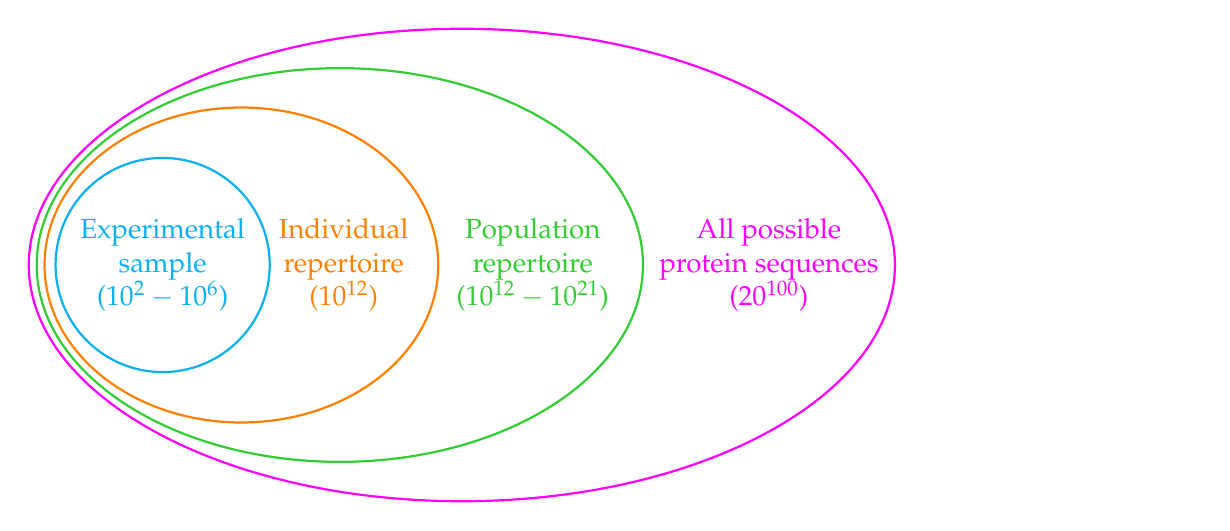
\begin{tikzpicture}
        \node [draw, circle, thick, ProcessBlue, minimum size=2cm, align=center] at   (0,0)   {Experimental\\sample\\($10^2 - 10^6$)};
        \node [draw, ellipse, thick, orange, minimum width=5cm, minimum height=4cm, align=center] at   (1,0) {};
        \node [minimum width=7cm, orange, minimum height=5cm, xshift=3mm, align=center] at   (2,0) {Individual\\repertoire\\($10^{12}$)};
        \node [draw, ellipse, thick, LimeGreen, minimum width=7.7cm, minimum height=5cm, align=center] at (2.25, 0) {};
        \node [minimum width=7cm, LimeGreen, minimum height=5cm, xshift=2.9cm, align=center] at (1.8, 0) {Population\\repertoire\\($10^{12} - 10^{21}$)};
         \node [draw, ellipse, thick, Fuchsia, minimum width=11cm, minimum height=6cm, align=center] at (3.8, 0) {};
         \node [Fuchsia, minimum width=11cm, minimum height=6cm, align=center, xshift=3.9cm] at (3.8, 0) {All possible \\protein sequences \\($20^{100}$)};
    \end{tikzpicture}


\end{frame}

\begin{frame}\frametitle{Example: discrete distribution}
\begin{itemize}
\item[]
Let $\mathcal X = \{{\color{orange} 1}, {\color{orange} 2}, {\color{orange} 4}\}$, 
$\mathcal Y = \{ {\color{ProcessBlue} 1}, {\color{ProcessBlue} 3}, {\color{ProcessBlue} 5}\}$ and define distributions $\color{red}\mu$ and $\color{blue}\nu$ via
\ba
{\color{red} \mu} ({\color{orange} 1}) & = 0.6, 
\ {\color{red} \mu} ({\color{orange} 2}) = 0.3, 
\ {\color{red} \mu} ({\color{orange} 4}) = 0.1 \\
{\color{blue} \nu} ({\color{ProcessBlue} 1}) & = 0.3, 
\ {\color{blue} \nu}({\color{ProcessBlue} 3}) = 0.5, 
\ {\color{blue} \nu}({\color{ProcessBlue} 5}) = 0.2.
\ea
\vspace{-2em}
\begin{center}
\includegraphics[width=0.8\linewidth]{Images/pmf.png}
\end{center}
\end{itemize}
\end{frame}

\begin{frame}\frametitle{Example: discrete distribution}
\begin{itemize}
\item[]
The cost matrix ${\color{Green} \mathbf D}_{{\color{orange} i}{\color{ProcessBlue} j}} = {\color{Green} d}({\color{orange} x_i}, {\color{ProcessBlue} y_j})$, using 
${\color{Green} d}({\color{orange} x}, {\color{ProcessBlue} y}) = |{\color{orange} x} - {\color{ProcessBlue} y}|$ as our metric, is
\ba
{\color{Green} \mathbf D} = 
	\begin{blockarray}{cccc}
	& {\color{ProcessBlue} 1} & {\color{ProcessBlue} 3} & {\color{ProcessBlue} 5} \\
	\begin{block}{c(ccc)}
		{\color{orange} 1} & |{\color{orange} 1} - {\color{ProcessBlue} 1}| & |{\color{orange} 1} - {\color{ProcessBlue} 3}| & |{\color{orange} 1} - {\color{ProcessBlue} 5}| \\
		{\color{orange} 2} & |{\color{orange} 2} - {\color{ProcessBlue} 1}| & |{\color{orange} 2} - {\color{ProcessBlue} 3}| & |{\color{orange} 2} - {\color{ProcessBlue} 5}| \\
		{\color{orange} 4} & |{\color{orange} 4} - {\color{ProcessBlue} 1}| & |{\color{orange} 4} - {\color{ProcessBlue} 3}| & |{\color{orange} 4} - {\color{ProcessBlue} 5}| \\
	\end{block}
\end{blockarray}
=
\begin{blockarray}{cccc}
	& {\color{ProcessBlue} 1} & {\color{ProcessBlue} 3} & {\color{ProcessBlue} 5} \\
	\begin{block}{c(ccc)}
		{\color{orange} 1} & \color{Green}0 & \color{Green}2 & \color{Green}4 \\
		{\color{orange} 2} & \color{Green}1 & \color{Green}1 & \color{Green}3 \\
		{\color{orange} 4} & \color{Green}3 & \color{Green}1 & \color{Green}1 \\
	\end{block}
\end{blockarray}
\ea
\vspace{-3em}
\begin{center}
\includegraphics[width=0.7\linewidth]{Images/pmf.png}
\end{center}
\end{itemize}
\end{frame}

\begin{frame}\frametitle{Example: "proof" by inspection}
\begin{minipage}{0.49\linewidth}
\begin{itemize}
\item
${\color{blue} \nu}$ needs 0.2 mass at $x = 5$;  the closest mass from ${\color{red} \mu}$ is 0.1 unit at $x = 4$
\item
${\color{blue} \nu}$ still needs 0.1 unit of mass for $x = 5$; get from ${\color{red} \mu}$ at next closest value, $x = 2$
\item
This leaves 0.2 units from ${\color{red} \mu}$ at $x = 2$ which can be moved to $x = 3$ for ${\color{blue} \nu}$
\item
Remaining 0.3 units needed at $x = 3$ for ${\color{blue} \nu}$ can be obtained from $x = 1$ in ${\color{red} \mu}$
\item
This leaves 0.3 units at $x = 1$ for ${\color{blue} \nu}$, as desired.
\end{itemize}
\end{minipage}
\begin{minipage}{0.49\linewidth}
\includegraphics[width=\linewidth]{Images/pmf.png}
\footnotesize
\vspace{-1em}
\ba
{\color{Purple} \mathbf P^*} & = \begin{blockarray}{cccc}
	& {\color{ProcessBlue} 1} & {\color{ProcessBlue} 3} & {\color{ProcessBlue} 5} \\
	\begin{block}{c(ccc)}
		{\color{orange} 1} & \color{Purple} 0.3 & \color{Purple} 0.3 & \color{Purple} 0 \\
		{\color{orange} 2} & \color{Purple} 0 & \color{Purple}  0.2 & \color{Purple} 0.1 \\
		{\color{orange} 4} & \color{Purple} 0 & \color{Purple} 0 & \color{Purple} 0.1 \\
	\end{block}
\end{blockarray} \\
\mathcal L_{{\color{Green} \mathbf D}}(\color{red}\mu, \color{blue}\nu) 
	& = \langle \mathbf {\color{Green} D}, {\color{Purple} \mathbf P^*} \rangle \\
	& = {\color{Green} 2} \cdot {\color{Purple} 0.3} + {\color{Green} 1} \cdot {\color{Purple} 0.2} + {\color{Green} 3} \cdot {\color{Purple} 0.1} + {\color{Green} 1} \cdot {\color{Purple} 0.1} \\
	& = 1.2
\ea
\end{minipage}
\end{frame}

\begin{frame}[fragile]\frametitle{Example: rigorous solution}
\small
To solve for ${\color{Purple} \mathbf P^*}$ rigorously, we can set up a linear program using the row-sums and column-sums constraints:
\bigskip
\ba
\;& \text{minimize} \ {\color{Purple} \mathbf P}_{1,2} + 4{\color{Purple} \mathbf P}_{1,3} + {\color{Purple} \mathbf P}_{2,1} +  {\color{Purple} \mathbf P}_{2, 2} + 3{\color{Purple} \mathbf P}_{2,3} + 3{\color{Purple} \mathbf P}_{3,1} + {\color{Purple} \mathbf P}_{3,2} + {\color{Purple} \mathbf P}_{3, 3} \\
& \text{subject to} \begin{cases}
	 {\color{Purple} \mathbf P}_{1,1} + {\color{Purple} \mathbf P}_{1,2} + {\color{Purple} \mathbf P}_{1,3} = 0.6 \\
	 {\color{Purple} \mathbf P}_{2,1} + {\color{Purple} \mathbf P}_{2,2} + {\color{Purple} \mathbf P}_{2,3} = 0.3 \\
	 {\color{Purple} \mathbf P}_{3,1} + {\color{Purple} \mathbf P}_{3,2} + {\color{Purple} \mathbf P}_{3,3} = 0.1 \\
	 {\color{Purple} \mathbf P}_{1,1} + {\color{Purple} \mathbf P}_{2,1} + {\color{Purple} \mathbf P}_{3,1} = 0.3 \\
	 {\color{Purple} \mathbf P}_{1,2} + {\color{Purple} \mathbf P}_{2,2} + {\color{Purple} \mathbf P}_{3,2} = 0.5 \\
	 {\color{Purple} \mathbf P}_{1,3} + {\color{Purple} \mathbf P}_{2,3} + {\color{Purple} \mathbf P}_{3,3} = 0.2 \\
	 0 \le {\color{Purple} \mathbf P}_{i,j} \le 1 \ \forall i,j 
\end{cases}
\ea
\end{frame}

\begin{frame}\frametitle{Wasserstein distance}
\begin{itemize}
\item[]
$
\mathcal L_{{\color{Green} d}}(
		{\color{red} \mu}, {\color{blue} \nu}) 
	\equiv \text{Wasserstein distance between ${\color{red} \mu}$ and ${\color{blue} \nu}$ w.r.t. ${\color{Green} d}$}
$
\bigskip
\item[]
Discrete case:
\ba
\mathcal L_{{\color{Green} \mathbf D}}(
		{\color{red} \mu}, {\color{blue} \nu})
	& = \min_{{\color{Purple} \mathbf P} \in \Pi({\color{red} \mu}, {\color{blue} \nu})}
		\sum_{i=1}^n \sum_{j=1}^m \mathbf {\color{Green} D}_{i,j} \mathbf {\color{Purple} \mathbf P}_{i,j}
\ea
where
$\mathbf {\color{Green} D}_{i,j} = {\color{Green} d}(x_i, y_j)$ 
and
$\mathbf {\color{Purple} \mathbf P}_{i,j} = {\color{violet} \pi}(x_i, y_j)$
\end{itemize}
\end{frame}

\begin{frame}\frametitle{Admissible couplings}
\begin{itemize}
\item
Write discrete distributions ${\color{red} \mu}, {\color{blue} \nu}$ as vectors ${\color{red} \mathbf r}, {\color{blue} \mathbf c}$ respectively.
\bigskip
\item
Set of admissible couplings:
\ba
\Pi({\color{red} \mathbf r}, {\color{blue} \mathbf c}) 
	= \set{ {\color{Purple} \mathbf P} \in \reals_+^{n \times m} : 
	\mathbf {\color{Purple} \mathbf P} \mathbf{1}_m = {\color{red} \mathbf r} \text{ and }
	\mathbf {\color{Purple} \mathbf P}^\mathsf{T} \mathbf{1}_n = {\color{blue} \mathbf c} }
\ea
\item Then
\begin{align}
\mathcal L_{{\color{Green} \mathbf D}}(
		{\color{red} \mathbf r}, {\color{blue} \mathbf c})
	& = \min_{{\color{Purple} \mathbf P} \in \Pi({\color{red} \mathbf r} , {\color{blue} \mathbf c})}
		\sum_{i=1}^n \sum_{j=1}^m \mathbf {\color{Green} D}_{i,j} \mathbf {\color{Purple} \mathbf P}_{i,j} \\
	& = \min_{{\color{Purple} \mathbf P} \in \Pi({\color{red} \mathbf r} , {\color{blue} \mathbf c})} 
		\langle \mathbf {\color{Green} D}, {\color{Purple} \mathbf P} \rangle 
\end{align}
is a linear program over a convex polytope
\medskip
\item
Complexity: $\mathcal O(k^3 \log k)$, $k = \max(n, m)$ 
\end{itemize}
\end{frame}

\begin{frame}\frametitle{Sinkhorn distance}
\begin{itemize}
\item
Cuturi (2013): let's regularize for high entropy of the couplings ${\color{Purple} \mathbf P}$ for simplicity
\bigskip
\item
In particular, they introduce the Sinkhorn distance 
\begin{align}
\mathcal L_{{\color{Green} \mathbf D}}^\lambda(
		{\color{red} \mathbf r}, {\color{blue} \mathbf c})
	:= \left\langle {\color{Green} \mathbf D}, {\color{Purple} \mathbf P}_{{\color{red} \mathbf r}, {\color{blue} \mathbf c}}^\lambda \right\rangle
\end{align}
where
\begin{align}
{\color{Purple} \mathbf P}_{{\color{red} \mathbf r}, {\color{blue} \mathbf c}}^\lambda 
= \argmin_{{\color{Purple} \mathbf P} \in \Pi({\color{red} \mathbf r} , {\color{blue} \mathbf c})}
	\left\{ \langle {\color{Green} \mathbf D}, {\color{Purple} \mathbf P} \rangle - \frac{1}{\lambda} h({\color{Purple} \mathbf P}) \right\}
\end{align}
and $h({\color{Purple} \mathbf P}) 
	:= - \sum_{i=1}^d \sum_{j=1}^d {\color{Purple} \mathbf P}_{i,j} \log({\color{Purple} \mathbf P}_{i,j})$ is the Shannon entropy of ${\color{Purple} \mathbf P}$.
\end{itemize}
\end{frame}

\begin{frame}\frametitle{What is Sinkhorn doing?}
\begin{itemize}
\item
Turns out we're constraining region to a new region $\Pi_\alpha$ with
\begin{align}
\Pi_\alpha({\color{red} \mathbf r} , {\color{blue} \mathbf c})
	= \left\{ {\color{Purple} \mathbf P} \in \Pi({\color{red} \mathbf r} , {\color{blue} \mathbf c}) : 
		\text{KL}\left({\color{Purple} \mathbf P} \ \big{|}\big| \ {\color{red} \mathbf r} {\color{blue} \mathbf c}^{\mathsf T} \right) \le \alpha \right\}.
\end{align}
so that
\ba
\mathcal L_{{\color{Green} \mathbf D}}^\lambda(
		{\color{red} \mathbf r}, {\color{blue} \mathbf c})
	= \min_{{\color{Purple} \mathbf P} \in \Pi_\alpha({\color{red} \mathbf r} , {\color{blue} \mathbf c})} 
		\langle \mathbf {\color{Green} D}, {\color{Purple} \mathbf P} \rangle 
\ea
\begin{center}
\includegraphics[width=0.7\linewidth]{Images/Polytope.png}
\end{center}

\end{itemize}

\end{frame}

\begin{frame}\frametitle{Fast OT via regularization}
\begin{minipage}{0.49\linewidth}
\begin{itemize}
\item
Discrete OT seeks minimum over convex polytope
\medskip
\begin{itemize}
\item
$\mathcal O(d^3 \log d)$, $d = \max(n, m)$
\end{itemize}
\bigskip
\item
Cuturi (2013): regularize space of couplings for high entropy
\medskip
\begin{itemize}
\item
Empirical tests suggest $\mathcal O(d)$ to $\mathcal O(d^2)$
\end{itemize}
\end{itemize}
\end{minipage}
\begin{minipage}{0.49\linewidth}
\begin{center}
\includegraphics[width=\linewidth]{Images/Sinkhorn_diagram.png}
\end{center}
\end{minipage}
\end{frame}


\begin{frame}\frametitle{TCRdist [Dash et al. '17]}
\begin{align}
\text{TCRdist}(r_1, r_2)
	& := \sum_{p \in \text{{\color{ProcessBlue} CDR positions}}} 
		\sum_{(a_1, a_2) \in p}
		{\color{Orange} w}(p) 
		\text{{\color{Green} AAdist}}(a_1, a_2; p)
\end{align}

where:
\footnotesize
\begin{itemize}
\item
$\text{{\color{ProcessBlue} CDR positions}} 
	:= \{\text{CDR1}\alpha, \text{CDR2}\alpha, \text{CDR2.5}\alpha, 
		\text{CDR3}\alpha,
		 \text{CDR1}\beta, \text{CDR2}\beta, \text{CDR2.5}\beta, \text{CDR3}\beta\}$
\item 
$ {\color{Orange} w}(p) := \begin{cases} 3, & p \in \{\text{CDR3}\alpha, \text{CDR3}\beta\} \\
						1, & \text{else}
		\end{cases}$
\item
$ \text{{\color{Green} AAdist}}(a_1, a_2; p) := 
\begin{cases}
	0, & a_1 = a_2 \\
	8, & a_1 = \text{`}\texttt{-}\text{'} \oplus a_2 = \text{`}\texttt{-}\text{'}, 
		\ p \in \{\text{CDR3}\alpha, \text{CDR3}\beta\} \\
	4, & a_1 = \text{`}\texttt{-}\text{'} \oplus a_2 = \text{`}\texttt{-}\text{'}, 
		\ p \not\in \{\text{CDR3}\alpha, \text{CDR3}\beta\} \\

	4 - \min(0,  \text{{\color{Purple} BLOSUM62}}(a_1, a_2)), & \text{else} 
\end{cases}$ 
\item
{\color{Purple} BLOSUM62}: widely-used AA substitution matrix
[Henikoff '92]
\end{itemize}
\end{frame}

\begin{frame}\frametitle{Z-scores for randomization vs replicate null}
\begin{center}
\includegraphics[width=0.75\linewidth]{Images/z_score_densities.pdf}
\end{center}
\end{frame}

\end{document}























